% TinyGPT paper, IEEE conference format. Compile on Overleaf (or any TeX Live) with:
%   pdflatex paper && bibtex paper && pdflatex paper && pdflatex paper
% Figures: architecture_wide.pdf and loss_curve.pdf (generate with make_figures.py).
% NOTE: this file was written without a local LaTeX install and has not been compiled by the author;
% paper.pdf (rendered from paper.html) is the checked version. Numbers match paper/eval_results.txt.
\documentclass[conference]{IEEEtran}
\usepackage{graphicx}
\usepackage{booktabs}
\usepackage{amsmath}
\usepackage{cite}
\usepackage{url}

\begin{document}

\title{TinyGPT: A Character-Level Transformer Language Model Trained from Scratch on Consumer Hardware}

\author{\IEEEauthorblockN{[Author Name]}
\IEEEauthorblockA{[Department, Institution]\\
[City, Country]\\
[email address]}}

\maketitle

\begin{abstract}
We present TinyGPT, a decoder-only transformer language model with 10.76 million parameters (6 layers, 6 attention heads,
384-dimensional embeddings, 256-character context), implemented from scratch in PyTorch and trained on the 1.1-million-character
Tiny Shakespeare corpus in 27 minutes on a laptop GPU. On the held-out split it reaches 1.50 nats/character (2.16 bits/character,
perplexity 4.47), compared with 2.48 nats for a character-bigram baseline and 4.17 for a uniform guess. We document the training
dynamics, including overfitting after roughly 41 passes over the data; measure how sampling temperature trades lexical validity
against diversity; and describe an interactive chat front end that frames user input as lines of a play script, together with
one-click launchers for Windows, macOS and Linux. The model imitates the style and formatting of its corpus but does not produce
coherent sentences, and we state the limitations of this single-run study.
\end{abstract}

\begin{IEEEkeywords}
language model, transformer, self-attention, character-level modeling, text generation
\end{IEEEkeywords}

\section{Introduction}
Transformer language models \cite{vaswani2017,radford2019} now underpin most text-generation systems, but their scale hides the
mechanisms involved. A model small enough to train on a laptop in under half an hour exposes the full pipeline---tokenization,
causal self-attention, optimization, sampling---to inspection and experiment. Our contributions are:
\begin{enumerate}
\item A from-scratch decoder-only transformer (Section~III) whose attention, blocks and sampler are written directly in
PyTorch \cite{paszke2019} without a transformer library.
\item An evaluation against uniform and bigram baselines on the complete held-out split, with an analysis of overfitting
(Section~V).
\item A measurement of how sampling temperature affects lexical validity and diversity of generated text.
\item An interactive ``play-script'' chat interface and launchers that select CUDA, Apple MPS or CPU automatically (Section~VI).
\end{enumerate}

\section{Related Work}
The transformer \cite{vaswani2017} replaced recurrence with self-attention; GPT-2 \cite{radford2019} showed that a decoder-only stack
trained for next-token prediction scales to broad text generation. Our design follows the compact style of nanoGPT \cite{karpathy2022}
and uses the Tiny Shakespeare corpus distributed with char-rnn \cite{karpathy2015}. Al-Rfou \emph{et al.} \cite{alrfou2019}
demonstrated that deep self-attention models operate effectively on characters. Individual components are standard: pre-layer
normalization \cite{xiong2020,ba2016}, residual connections \cite{he2016}, GELU activations \cite{hendrycks2016}, weight tying
\cite{press2017}, dropout \cite{srivastava2014}, and AdamW \cite{loshchilov2019}. Generation uses temperature scaling with top-$k$
truncation \cite{fan2018}; nucleus sampling \cite{holtzman2020} is a common alternative that we do not evaluate.

\section{Model Architecture}
The model maps character indices $x_{1..T}$ ($T\le 256$) to logits over a 65-symbol vocabulary. The input is the sum of a token
embedding and a learned absolute position embedding, followed by dropout:
\begin{equation}
h_0 = \mathrm{Dropout}(E[x] + P[0..T{-}1]).
\end{equation}
Each of the $L=6$ blocks applies pre-LayerNorm self-attention and a feed-forward network, each with a residual connection:
\begin{equation}
h' = h + \mathrm{MHA}(\mathrm{LN}(h)),\quad h'' = h' + \mathrm{MLP}(\mathrm{LN}(h')).
\end{equation}
Attention uses 6 heads of dimension 64; queries, keys and values come from one fused linear layer ($384\to1152$, no bias):
\begin{equation}
\mathrm{Attn}(Q,K,V)=\mathrm{softmax}\!\left(\frac{QK^{\top}}{\sqrt{d_k}}+M\right)V,
\end{equation}
where $M_{ij}=0$ for $j\le i$ and $-\infty$ otherwise. Dropout (0.2) is applied to the attention weights and output. The MLP is
$384\to1536\to384$ with GELU and dropout on its output. A final LayerNorm precedes a linear layer that shares its weights with the
token embedding \cite{press2017}:
\begin{equation}
\mathrm{logits}=\mathrm{LN}_f(h_L)\,E^{\top}.
\end{equation}
Weights are initialized from $\mathcal{N}(0,0.02^2)$ with zero biases. The model has 10,761,600 parameters (Table~\ref{tab:params});
with only 65 symbols the embeddings are negligible and 98.9\% of the parameters are in the blocks.

\begin{figure*}[t]
\centering
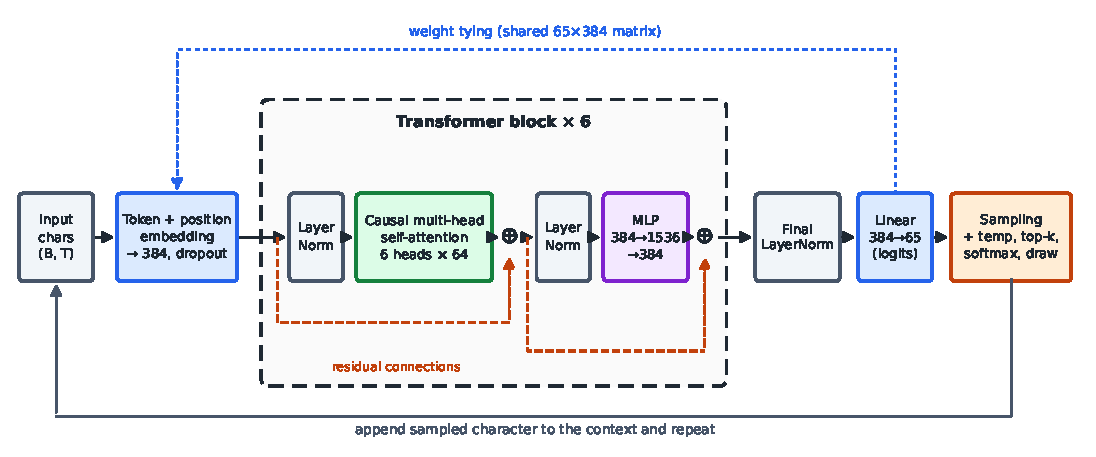
\includegraphics[width=\textwidth]{architecture_wide.pdf}
\caption{TinyGPT architecture. Token and learned position embeddings feed six identical pre-LayerNorm transformer blocks (causal
self-attention and MLP, each with a residual connection). A final LayerNorm and linear layer produce logits over 65 characters; the
linear layer shares its weights with the token embedding. Sampled characters are appended to the context.}
\label{fig:arch}
\end{figure*}

\begin{table}[t]
\caption{Parameter breakdown}\label{tab:params}
\centering\small
\begin{tabular}{lr}
\toprule
Component & Parameters\\
\midrule
Token embedding (tied with output layer) & 24,960\\
Position embedding & 98,304\\
Per block: attention (QKV + projection) & 589,824\\
Per block: MLP & 1,181,568\\
Per block: two LayerNorms & 1,536\\
\quad Block total ($\times6=10{,}637{,}568$) & 1,772,928\\
Final LayerNorm & 768\\
\midrule
\textbf{Total} & \textbf{10,761,600}\\
\bottomrule
\end{tabular}
\end{table}

\section{Training Setup}
\subsection{Data and objective}
We use Tiny Shakespeare \cite{karpathy2015}: 1,115,394 characters with 65 distinct symbols, tokenized at the character level. The first
90\% (1,003,854 characters) is used for training and the final 10\% (111,540 characters) for validation; the split is contiguous and
unshuffled. The objective is cross-entropy on next-character prediction with targets shifted by one position.
\subsection{Optimization}
Each step samples 32 random 256-character windows (8,192 tokens). We use AdamW \cite{loshchilov2019} at a constant learning rate of
$3\times10^{-4}$ (default weight decay 0.01) with gradient-norm clipping at 1.0 and no warmup or decay. Training ran for 5,000 steps
(40.96\,M tokens, about 41 passes over the training split). Every 250 steps, validation loss was estimated on 50 random batches and the
checkpoint saved when it improved. The seed was fixed (1337). Hardware: Apple M1 Pro, 32\,GB, PyTorch 2.15 (MPS), fp32; wall-clock
time 1,640\,s ($\approx$0.33\,s/step).

\section{Experiments and Results}
\subsection{Language-modeling quality}
Training loss fell from 4.20 at initialization---close to $\ln 65=4.17$---to 1.13 at step 5,000 (Fig.~\ref{fig:loss}). The periodic
validation estimate reached its minimum of 1.48 at step 4,000 and then drifted to 1.49 while training loss kept falling, a standard
signature of overfitting. The step-4,000 checkpoint was kept. Re-evaluating it on the entire validation split with non-overlapping
256-character windows (111,360 characters scored) gives Table~\ref{tab:loss}, with uniform and character-bigram (add-one) baselines
trained on the same split. TinyGPT reduces the loss by 40\% relative to the bigram model.

\begin{table}[t]
\caption{Held-out loss on the full validation split}\label{tab:loss}
\centering\small
\begin{tabular}{lrrr}
\toprule
Model & nats/char & bits/char & Perplexity\\
\midrule
Uniform & 4.174 & 6.022 & 65.00\\
Bigram (add-one) & 2.482 & 3.581 & 11.96\\
\textbf{TinyGPT (this work)} & \textbf{1.498} & \textbf{2.160} & \textbf{4.47}\\
\bottomrule
\end{tabular}
\end{table}

\begin{figure}[t]
\centering
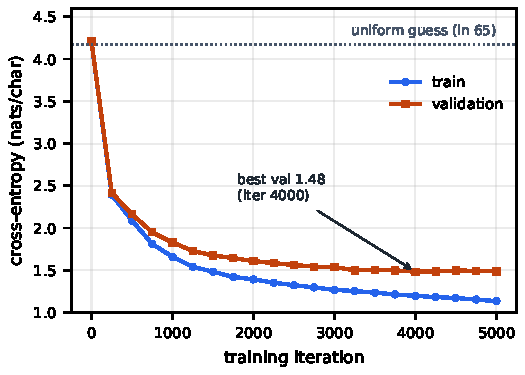
\includegraphics[width=\columnwidth]{loss_curve.pdf}
\caption{Training and validation loss (50-batch estimates logged every 250 steps). The validation minimum (1.48) occurs at step 4,000.}
\label{fig:loss}
\end{figure}

\subsection{Effect of sampling temperature}
We generated 8 sequences of 1,000 characters at each temperature (top-$k=40$, fixed seed) and measured the share of generated words
found in the training split and the share of distinct word tokens (Table~\ref{tab:temp}). Low temperature yields almost only valid
words but repeats them heavily; high temperature increases diversity at the cost of invented words. Validity can exceed the 94.3\% of
real held-out words found in the training vocabulary because low-temperature text over-uses frequent words; the metric measures
spelling, not grammaticality or meaning.

\begin{table}[t]
\caption{Generated-word statistics by temperature}\label{tab:temp}
\centering\small
\begin{tabular}{rrrr}
\toprule
Temp. & Words & In train vocab. & Distinct\\
\midrule
0.5 & 1,582 & 99.1\% & 22.9\%\\
0.8 & 1,560 & 96.2\% & 33.8\%\\
1.0 & 1,490 & 93.2\% & 39.3\%\\
1.2 & 1,399 & 87.4\% & 48.9\%\\
\bottomrule
\end{tabular}
\end{table}

\subsection{Qualitative samples}
At temperature 0.8 the model reproduces speaker labels, colons, line breaks and archaic vocabulary, but sentences are not coherent:
\begin{quote}\small\ttfamily
ROMEO:\\
I think, there an extremest is my friends,\\
For your fortune of battle persons,\\
Being the bloody of the plague,
\end{quote}

\section{Interactive Interface and Deployment}
\textbf{Chat.} The model is a text continuer, not an instruction-following assistant. We frame the conversation as a play script: the
user's message is appended as a speech by one character, followed by the other character's label, and the model generates until it
emits a blank line, which ends a speech in the training data. Memory is limited by the 256-character context window.

\textbf{Portability.} The code selects CUDA, Apple MPS or CPU automatically. Windows batch files (and a shell script for macOS and Linux)
create a virtual environment, install PyTorch (the CUDA build when an NVIDIA GPU is detected) and start chat, generation or training;
the trained checkpoint (44.6\,MB) is distributed with the code. Source code, checkpoint, training log and figure scripts:
\url{https://github.com/MouryaGowd/TinyLLM}.

\section{Limitations}
Results come from a single run and seed, with no variance or ablations. The validation split both selects the checkpoint and reports
its loss, so Table~\ref{tab:loss} is slightly optimistic; there is no separate test set. A 10.8\,M-parameter model trained on 1\,M
characters cannot acquire semantic competence. The lexical-validity metric does not assess grammar or meaning, and there is no human
evaluation. We do not compare against other architectures or tokenizers, and the CUDA and CPU paths were not benchmarked.

\section{Conclusion}
We built and trained a 10.76\,M-parameter character-level GPT from scratch on a laptop in 27 minutes. It reaches 1.50 nats/character on
held-out text, a 40\% loss reduction over a bigram baseline, and learns the format and vocabulary of its corpus while overfitting after
about 40 epochs. Natural extensions are subword tokenization, a learning-rate schedule, a larger corpus, a held-out test set, and
instruction fine-tuning.

\begin{thebibliography}{15}
\bibitem{vaswani2017} A. Vaswani \emph{et al.}, ``Attention is all you need,'' in \emph{Advances in Neural Information Processing Systems 30}, 2017.
\bibitem{radford2019} A. Radford, J. Wu, R. Child, D. Luan, D. Amodei, and I. Sutskever, ``Language models are unsupervised multitask learners,'' OpenAI, Tech. Rep., 2019.
\bibitem{karpathy2022} A. Karpathy, ``nanoGPT,'' GitHub repository, 2022. [Online]. Available: \url{https://github.com/karpathy/nanoGPT}
\bibitem{karpathy2015} A. Karpathy, ``char-rnn (Tiny Shakespeare dataset),'' GitHub repository, 2015. [Online]. Available: \url{https://github.com/karpathy/char-rnn}
\bibitem{alrfou2019} R. Al-Rfou, D. Choe, N. Constant, M. Guo, and L. Jones, ``Character-level language modeling with deeper self-attention,'' in \emph{Proc. AAAI Conf. Artificial Intelligence}, 2019.
\bibitem{xiong2020} R. Xiong \emph{et al.}, ``On layer normalization in the transformer architecture,'' in \emph{Proc. Int. Conf. Machine Learning (ICML)}, 2020.
\bibitem{press2017} O. Press and L. Wolf, ``Using the output embedding to improve language models,'' in \emph{Proc. Conf. European Chapter of the ACL (EACL)}, 2017.
\bibitem{hendrycks2016} D. Hendrycks and K. Gimpel, ``Gaussian error linear units (GELUs),'' arXiv:1606.08415, 2016.
\bibitem{loshchilov2019} I. Loshchilov and F. Hutter, ``Decoupled weight decay regularization,'' in \emph{Proc. Int. Conf. Learning Representations (ICLR)}, 2019.
\bibitem{srivastava2014} N. Srivastava, G. Hinton, A. Krizhevsky, I. Sutskever, and R. Salakhutdinov, ``Dropout: A simple way to prevent neural networks from overfitting,'' \emph{J. Mach. Learn. Res.}, vol. 15, 2014.
\bibitem{fan2018} A. Fan, M. Lewis, and Y. Dauphin, ``Hierarchical neural story generation,'' in \emph{Proc. Annu. Meeting Assoc. Computational Linguistics (ACL)}, 2018.
\bibitem{holtzman2020} A. Holtzman, J. Buys, L. Du, M. Forbes, and Y. Choi, ``The curious case of neural text degeneration,'' in \emph{Proc. ICLR}, 2020.
\bibitem{paszke2019} A. Paszke \emph{et al.}, ``PyTorch: An imperative style, high-performance deep learning library,'' in \emph{Advances in Neural Information Processing Systems 32}, 2019.
\bibitem{ba2016} J. L. Ba, J. R. Kiros, and G. E. Hinton, ``Layer normalization,'' arXiv:1607.06450, 2016.
\bibitem{he2016} K. He, X. Zhang, S. Ren, and J. Sun, ``Deep residual learning for image recognition,'' in \emph{Proc. IEEE Conf. Computer Vision and Pattern Recognition (CVPR)}, 2016.
\end{thebibliography}

\end{document}
